\documentclass{article}
\usepackage[T1]{fontenc}
\usepackage[preprint]{colm2026_conference}

\usepackage{microtype}
\usepackage{hyperref}
\usepackage{url}
\usepackage{booktabs}
\usepackage{graphicx}
\usepackage{amsmath,amssymb}
\usepackage{float}
\usepackage{xcolor}
\definecolor{citeblue}{rgb}{0.16, 0.42, 0.73}
\hypersetup{colorlinks=true, citecolor=citeblue, linkcolor=citeblue, urlcolor=citeblue}
\usepackage[capitalize,noabbrev]{cleveref}

% Generated by src/analysis.py. Do not edit by hand.
\newcommand{\LambdaMed}{0.3}
\newcommand{\aHatMax}{1.97}
\newcommand{\aHatMed}{0.69}
\newcommand{\aHatMin}{0.13}
\newcommand{\aStarMed}{2.6}
\newcommand{\bestCfgScale}{2.9}
\newcommand{\bestCfgView}{HM10, image normal, f/1.8}
\newcommand{\blurMedCm}{0.31}
\newcommand{\burstMaxMs}{500}
\newcommand{\burstMedianMs}{100}
\newcommand{\burstMinMs}{3}
\newcommand{\dMedAll}{3.6}
\newcommand{\dMedAllHi}{3.7}
\newcommand{\dMedAllLo}{3.4}
\newcommand{\dMedExpFive}{2.9}
\newcommand{\dMedExpFour}{4.7}
\newcommand{\dMedExpSeven}{3.4}
\newcommand{\dMedExpTen}{3.4}
\newcommand{\fgwMax}{1.01}
\newcommand{\fgwMin}{0.14}
\newcommand{\fwhmPxCfgMax}{13}
\newcommand{\fwhmPxCfgMin}{8}
\newcommand{\ipBestMax}{1127}
\newcommand{\ipBestMin}{606}
\newcommand{\ipCandMin}{400}
\newcommand{\ipMax}{1127}
\newcommand{\ipMin}{402}
\newcommand{\lEffM}{5.34}
\newcommand{\lEffQHi}{5.53}
\newcommand{\lEffQLo}{4.99}
\newcommand{\lkAgreeMed}{+0.23}
\newcommand{\lkRatioMed}{0.13}
\newcommand{\lkShotRho}{+0.49}
\newcommand{\nArchiveShots}{15{,}969}
\newcommand{\nCampaigns}{4}
\newcommand{\nCfgPx}{6}
\newcommand{\nConfigs}{23}
\newcommand{\nConfigsOwn}{6}
\newcommand{\nExpFive}{9}
\newcommand{\nExpFour}{37}
\newcommand{\nExpSeven}{105}
\newcommand{\nExpTen}{142}
\newcommand{\nFramesProcessedM}{3.5}
\newcommand{\nLEff}{311}
\newcommand{\nOkBurst}{375}
\newcommand{\nOkCurrent}{421}
\newcommand{\nOkFlatTop}{404}
\newcommand{\nOwnCampEight}{1}
\newcommand{\nOwnCampNine}{1}
\newcommand{\nOwnCampSeven}{1}
\newcommand{\nOwnCampSix}{3}
\newcommand{\nShotsBestCfgL}{37}
\newcommand{\nShotsCalTotal}{355}
\newcommand{\nShotsCandidates}{368}
\newcommand{\nShotsElmy}{111}
\newcommand{\nShotsFetched}{368}
\newcommand{\nShotsL}{183}
\newcommand{\nShotsOwnScale}{241}
\newcommand{\nShotsProcessed}{352}
\newcommand{\nShotsSlowFps}{16}
\newcommand{\nShotsStats}{294}
\newcommand{\nStripBurst}{427}
\newcommand{\nStripShots}{468}
\newcommand{\nStripTenUs}{419}
\newcommand{\nTeAssumed}{234}
\newcommand{\nTeMeasured}{60}
\newcommand{\nTracksAll}{930{,}081}
\newcommand{\nTracksSel}{86{,}042}
\newcommand{\nWithinShot}{326}
\newcommand{\nXcorr}{175}
\newcommand{\outwardMed}{81}
\newcommand{\rhoDExp}{-0.13}
\newcommand{\rhoDFgw}{+0.07}
\newcommand{\rhoDIp}{+0.08}
\newcommand{\rhoDNbi}{+0.22}
\newcommand{\rhoVExp}{-0.01}
\newcommand{\rhoVFgw}{-0.08}
\newcommand{\rhoVIp}{-0.03}
\newcommand{\rhoVNbi}{-0.11}
\newcommand{\scaleCampEight}{5.2}
\newcommand{\scaleCampEightHi}{11.5}
\newcommand{\scaleCampEightLo}{3.6}
\newcommand{\scaleCampEightN}{32}
\newcommand{\scaleCampEightRho}{-0.58}
\newcommand{\scaleCampNine}{2.9}
\newcommand{\scaleCampNineHi}{4.2}
\newcommand{\scaleCampNineLo}{2.5}
\newcommand{\scaleCampNineN}{48}
\newcommand{\scaleCampNineRho}{-0.72}
\newcommand{\scaleCampSeven}{3.3}
\newcommand{\scaleCampSevenHi}{3.8}
\newcommand{\scaleCampSevenLo}{3.0}
\newcommand{\scaleCampSevenN}{22}
\newcommand{\scaleCampSevenRho}{-0.88}
\newcommand{\scaleCampSix}{3.7}
\newcommand{\scaleCampSixHi}{4.1}
\newcommand{\scaleCampSixLo}{3.3}
\newcommand{\scaleCampSixN}{253}
\newcommand{\scaleCampSixRho}{-0.64}
\newcommand{\scaleCfgCampEight}{5.2}
\newcommand{\scaleCfgCampEightHi}{11.5}
\newcommand{\scaleCfgCampEightLo}{3.6}
\newcommand{\scaleCfgCampEightN}{32}
\newcommand{\scaleCfgCampEightRho}{-0.58}
\newcommand{\scaleCfgCampEightView}{photron HM10 f/2.8  4.8mm   nd 0.9}
\newcommand{\scaleCfgCampNine}{2.7}
\newcommand{\scaleCfgCampNineHi}{3.4}
\newcommand{\scaleCfgCampNineLo}{2.5}
\newcommand{\scaleCfgCampNineN}{38}
\newcommand{\scaleCfgCampNineRho}{-0.82}
\newcommand{\scaleCfgCampNineView}{photron HM10 + Dalpha filter}
\newcommand{\scaleCfgCampSeven}{3.3}
\newcommand{\scaleCfgCampSevenHi}{3.8}
\newcommand{\scaleCfgCampSevenLo}{3.0}
\newcommand{\scaleCfgCampSevenN}{22}
\newcommand{\scaleCfgCampSevenRho}{-0.88}
\newcommand{\scaleCfgCampSevenView}{photron HM10}
\newcommand{\scaleCfgCampSix}{2.9}
\newcommand{\scaleCfgCampSixHi}{3.0}
\newcommand{\scaleCfgCampSixLo}{2.7}
\newcommand{\scaleCfgCampSixN}{70}
\newcommand{\scaleCfgCampSixRho}{-0.94}
\newcommand{\scaleCfgCampSixView}{HM10, image normal, f/1.8}
\newcommand{\scaleOwnMax}{5.2}
\newcommand{\scaleOwnMin}{2.7}
\newcommand{\scaleOwnRatio}{1.9}
\newcommand{\scaleOwnRhoStrong}{$-0.94$}
\newcommand{\scaleOwnRhoWeak}{$-0.58$}
\newcommand{\slBDFgw}{-0.14}
\newcommand{\slBDFgwHi}{+0.00}
\newcommand{\slBDFgwLo}{-0.41}
\newcommand{\slBDIp}{+0.25}
\newcommand{\slBDIpHi}{+1.11}
\newcommand{\slBDIpLo}{-0.13}
\newcommand{\slBVFgw}{-0.10}
\newcommand{\slBVFgwHi}{+0.12}
\newcommand{\slBVFgwLo}{-0.26}
\newcommand{\slBVIp}{-0.29}
\newcommand{\slBVIpHi}{+0.66}
\newcommand{\slBVIpLo}{-1.02}
\newcommand{\slDExp}{-0.16}
\newcommand{\slDExpHi}{+0.01}
\newcommand{\slDExpLo}{-0.35}
\newcommand{\slDFgw}{+0.06}
\newcommand{\slDFgwHi}{+0.21}
\newcommand{\slDFgwLo}{-0.08}
\newcommand{\slDIp}{+0.10}
\newcommand{\slDIpHi}{+0.40}
\newcommand{\slDIpLo}{-0.21}
\newcommand{\slDNbi}{+0.05}
\newcommand{\slDNbiHi}{+0.07}
\newcommand{\slDNbiLo}{+0.01}
\newcommand{\slVExp}{-0.01}
\newcommand{\slVExpHi}{+0.11}
\newcommand{\slVExpLo}{-0.12}
\newcommand{\slVFgw}{-0.06}
\newcommand{\slVFgwHi}{+0.05}
\newcommand{\slVFgwLo}{-0.18}
\newcommand{\slVIp}{-0.05}
\newcommand{\slVIpHi}{+0.19}
\newcommand{\slVIpLo}{-0.29}
\newcommand{\slVNbi}{-0.01}
\newcommand{\slVNbiHi}{+0.01}
\newcommand{\slVNbiLo}{-0.03}
\newcommand{\slowFpsKhz}{50}
\newcommand{\teDefault}{30}
\newcommand{\vHatMed}{0.06}
\newcommand{\vMedAll}{424}
\newcommand{\vMedAllHi}{439}
\newcommand{\vMedAllLo}{406}
\newcommand{\vMedExpFive}{359}
\newcommand{\vMedExpFour}{542}
\newcommand{\vMedExpSeven}{403}
\newcommand{\vMedExpTen}{419}
\newcommand{\vStarMed}{7345}
\newcommand{\vdRhoMed}{+0.07}
\newcommand{\vdRhoPooled}{+0.05}
\newcommand{\vdSlopeExpFive}{+0.18}
\newcommand{\vdSlopeExpFiveHi}{+0.35}
\newcommand{\vdSlopeExpFiveLo}{+0.14}
\newcommand{\vdSlopeExpFour}{+0.07}
\newcommand{\vdSlopeExpFourHi}{+0.16}
\newcommand{\vdSlopeExpFourLo}{-0.04}
\newcommand{\vdSlopeExpSeven}{+0.05}
\newcommand{\vdSlopeExpSevenHi}{+0.11}
\newcommand{\vdSlopeExpSevenLo}{+0.01}
\newcommand{\vdSlopeExpTen}{+0.16}
\newcommand{\vdSlopeExpTenHi}{+0.27}
\newcommand{\vdSlopeExpTenLo}{+0.11}
\newcommand{\vdSlopeMed}{+0.11}
\newcommand{\vdSlopeMedHi}{+0.15}
\newcommand{\vdSlopeMedLo}{+0.08}
\newcommand{\vdSlopePooled}{+0.09}
\newcommand{\vdSlopePooledBlur}{+0.05}
\newcommand{\vdSlopePooledBlurHi}{+0.07}
\newcommand{\vdSlopePooledBlurLo}{+0.03}
\newcommand{\vdSlopePooledHi}{+0.11}
\newcommand{\vdSlopePooledLo}{+0.06}
\newcommand{\vdSlopePosShare}{70}
\newcommand{\vxPxCfgMax}{1.40}
\newcommand{\vxPxCfgMin}{1.15}
\newcommand{\windowMedianMs}{186}
\newcommand{\withinScaleMax}{10284.3}
\newcommand{\withinScaleMaxLog}{4}
\newcommand{\withinScaleMed}{5.8}
\newcommand{\withinScaleMin}{0.4}
\newcommand{\withinScaleQHi}{13.6}
\newcommand{\withinScaleQLo}{3.8}
\newcommand{\xcorrRatioHi}{0.68}
\newcommand{\xcorrRatioLo}{0.52}
\newcommand{\xcorrRatioMed}{0.63}
\newcommand{\xcorrShotRho}{+0.29}
\newcommand{\xcorrVMed}{257}


\title{Radial Velocity and Size of Scrape-Off-Layer Filaments\\Across \nShotsStats{} MAST Discharges from 100~kHz Visible Imaging}

\author{Jessie Dong \\
Stanford University}

\begin{document}
\maketitle
\lhead{}
\renewcommand{\footrulewidth}{1.5pt}

\begin{abstract}
Filaments carry much of the cross-field transport in the tokamak scrape-off layer, and models predict how their radial velocity scales with their size. We measure both on MAST from the 100~kHz, $48 \times 256$ pixel strip recordings of the midplane fast camera in the public FAIR-MAST archive. An automatic pipeline built from standard computer-vision operations (running-minimum background, robust thresholding, connected components, Hungarian linking, least-squares tracks, and optical flow) produces \nTracksSel{} filament tracks in \nShotsStats{} discharges across four campaigns. The archive distributes no spatial calibration for these recordings; we recover the pixel scale for each camera configuration by regressing the image column of the plasma limb on the EFIT outboard LCFS radius across discharges, with bootstrap intervals, and obtain \scaleOwnMin{}--\scaleOwnMax{}~mm per pixel. The median radial velocity is \vMedAll{}~m/s and the median radial width is \dMedAll{}~cm. After correction for exposure blur, the velocity--width relation has a log--log slope of \vdSlopePooledBlur{} (95\% interval \vdSlopePooledBlurLo{} to \vdSlopePooledBlurHi), so the velocity is nearly independent of size over the measured range. In two-region units the filaments span $\hat a = \aHatMin$--$\aHatMax$, straddling the model's velocity maximum, which accounts for the flat dependence; but their normalized velocity is $\hat v \approx \vHatMed$, far below the model scale. Code and derived data are released.

\end{abstract}

\section{Introduction}
\label{sec:intro}

Filaments are field-aligned structures of excess density and temperature that form near the last closed flux surface (LCFS) of a tokamak and move radially outward through the scrape-off layer (SOL), carrying a large part of the cross-field particle and heat flux in the SOL \citep{krasheninnikov2001scrape, zweben2007edge, dippolito2011convective}. Their radial velocity sets how far they travel before they drain to the divertor targets and thereby the load on the first wall, and analytic models give this velocity as a function of filament size and of the parameters that control how the polarization charge of the filament is dissipated. When the charge drains through the sheath at the target, the velocity falls with size as $v \propto a^{-2}$ \citep{krasheninnikov2001scrape}, and when ion polarization current closes the circuit inside the filament, the velocity rises with size as $v \propto a^{1/2}$ \citep{garcia2006fluctuations}. The two-region model of \citet{myra2006collisionality} joins these limits and predicts a velocity maximum at a critical size $a^*$ set by the sound speed, the connection length, and the collisionality.

Testing these predictions requires velocities and sizes for many filaments under known plasma conditions, and on the Mega Amp Spherical Tokamak (MAST) the main instrument for this purpose has been a Photron SA1.1 fast camera that views the outboard midplane in visible light. Earlier MAST studies used wide-angle views, identified filaments by hand or with detection software built for that view, and worked from a small number of discharges \citep{dudson2008experiments, benayed2009interelm, kirk2016filaments, farley2019identification}, each requiring a camera calibration model fitted to the view in use.

The FAIR-MAST archive \citep{jackson2024fairmast} makes the full MAST data set public and includes a recording mode of the midplane camera that earlier work did not use at scale, a $48 \times 256$ pixel strip through the outboard edge recorded at 100{,}000 frames per second. The strip resolves radial motion at 10~$\mu$s intervals but spans only 48 rows, so it constrains radial motion and radial size and little else, and because the archive includes no spatial calibration for these recordings, the pixel scale has to be recovered from the data.

Here those recordings are turned into filament statistics with an automatic pipeline built from standard computer-vision operations, namely a running-minimum background model, robust thresholding, connected-component detection, Hungarian frame-to-frame assignment, least-squares track fitting, and Lucas--Kanade optical flow as an independent velocity estimate. The pixel scale is calibrated against the equilibrium reconstruction, since the image column of the plasma limb moves with the EFIT outboard LCFS radius from shot to shot. A robust regression over a campaign then gives the scale in millimetres per pixel with a bootstrap confidence interval for each camera configuration, using only the images and EFIT, and the pipeline is run on every usable strip recording in the archive.

Applied to the archive, the pipeline yields radial velocity and radial width for \nTracksSel{} filament tracks in \nShotsStats{} MAST discharges, with a median radial velocity of \vMedAll{}~m/s, a median radial full width at half maximum of \dMedAll{}~cm, and \outwardMed\% of tracks moving outward. The pooled velocity--size slope is $\vdSlopePooled$ in log--log units and $\vdSlopePooledBlur$ after the widths are corrected for exposure blur, so the velocity is nearly independent of size over the measured range, and in two-region units the filaments sit at $\hat a \approx \aHatMin$--$\aHatMax$, where the model places its velocity maximum, although their normalized velocity $\hat v \approx \vHatMed$ is far below the model scale. Robust regression gives the dependences of the per-shot median velocity and width on plasma current, Greenwald fraction, and beam power with confidence intervals, and code and derived data accompany the paper.

\section{Background}
\label{sec:background}

\paragraph{Filament motion.}
A filament is a field-aligned tube of plasma, with a cross-field radius $a$ between a few ion gyroradii and a few centimetres, that is denser and hotter than the surrounding SOL. In the outboard SOL the magnetic curvature and gradient drifts separate ions and electrons across the filament, and the resulting electric field drives an $E \times B$ drift that moves the whole filament radially outward \citep{krasheninnikov2001scrape, dippolito2011convective}. The drift speed depends on the potential that the charge separation can build, and therefore on the paths through which the polarization charge is dissipated, which leads to two standard limits. If the filament is connected along the field line to the divertor target, the charge drains through the sheath and $v \propto c_s (L_\parallel/R)(\rho_s/a)^2$, where $c_s$ is the sound speed, $\rho_s$ the ion sound gyroradius, $L_\parallel$ the connection length, and $R$ the major radius \citep{krasheninnikov2001scrape}, whereas if the ion polarization current closes the circuit inside the filament, $v \propto c_s (a/R)^{1/2}$ \citep{garcia2006fluctuations}.

\paragraph{The two-region model.}
\citet{myra2006collisionality} model the midplane and the divertor leg as two coupled regions and join these limits. With
\begin{equation}
    a^* = \rho_s^{4/5} L_\parallel^{2/5} R^{-1/5}, \qquad
    v^* = c_s \left(\frac{2 a^*}{R}\right)^{1/2}, \qquad
    \Theta = \left(\frac{a}{a^*}\right)^{5/2}, \qquad
    \Lambda = \frac{\nu_{ei} L_\parallel}{\Omega_e \rho_s},
    \label{eq:tworegion}
\end{equation}
and $\hat a = a/a^*$, $\hat v = v/v^*$, the model gives
\begin{equation}
    \hat v =
    \begin{cases}
        \hat a^{1/2} & \text{connected ideal interchange } (\Lambda < 1,\ \Theta < 1), \\
        \hat a^{-2} & \text{sheath connected } (\Lambda < 1,\ \Theta > 1), \\
        \Lambda\, \hat a^{-2} & \text{resistive X-point } (1 < \Lambda < \Theta), \\
        \hat a^{1/2} & \text{resistive ballooning } (\Lambda > 1,\ \Lambda > \Theta).
    \end{cases}
    \label{eq:regimes}
\end{equation}
Here $\nu_{ei}$ is the electron--ion collision frequency and $\Omega_e$ the electron gyrofrequency \citep{dippolito2011convective}, and at low collisionality the velocity rises as $\hat a^{1/2}$ for small filaments, peaks near $\hat a = 1$, and falls as $\hat a^{-2}$ for large ones. The model is a scaling argument whose prefactors depend on the filament profile and on the parallel structure, and simulations in realistic geometry find velocities below the model values by factors of order unity \citep{easy2014three, walkden2015characterization, paruta2018blob}. \citet{theiler2009blob} measured the velocity--size relation on the TORPEX basic plasma device and recovered the predicted transitions between regimes.

\paragraph{Camera measurements.}
Visible-light imaging records line-integrated $D_\alpha$ emission, which depends on the local density, temperature, and neutral density. Filaments appear as bright, field-aligned streaks against the quiescent background, and their emission tracks the density perturbation closely enough that velocities and widths from imaging agree with probe measurements within tens of percent \citep{zweben2007edge, benayed2009interelm}. In a tangential view the brightest image feature is the plasma limb, the band where the line of sight is tangent to the flux surfaces near the LCFS, and filaments cross the limb as they move outward. Because the camera integrates over each exposure, a filament that moves a distance $v\,t_{\rm exp}$ during the exposure is smeared by that distance along its direction of motion, an effect treated explicitly in Section~\ref{sec:analysis}.

\section{Data}
\label{sec:data}

\paragraph{Archive.}
FAIR-MAST \citep{jackson2024fairmast} serves the MAST data set as one Zarr store per discharge over HTTP, with a metadata API for discovering signals and shot parameters. The archive covers \nArchiveShots{} discharges. We read six groups from it: the midplane fast camera (\texttt{rbb}), the EFIT equilibrium reconstruction (\texttt{efm}), the summary signals for line-averaged density and Greenwald density (\texttt{esm}), the interferometer (\texttt{ane}), the core and edge Thomson scattering systems (\texttt{ayc}, \texttt{aye}), and the midplane $D_\alpha$ monitor (\texttt{xim}). Plasma current, heating scheme, injected beam power, and the flat-top interval come from the per-shot metadata table.

\paragraph{Camera.}
The \texttt{rbb} signal is the Photron SA1.1 fast camera (``bullet camera B'') at the HM10 midplane port, which views the outboard edge tangentially \citep{kirk2016filaments, farley2019identification}. In the recording mode we use, the camera reads out a $48 \times 256$ pixel region of its sensor at 100{,}000 frames per second with 10-bit depth; the region offset on the sensor is recorded with each shot. Exposure times are 1--10~$\mu$s, with 4, 7, and 10~$\mu$s the common settings. The metadata view string records the lens, aperture, and filter in use and whether the camera was mounted inverted; the SOL-side detection in Section~\ref{sec:method} makes the pipeline independent of this orientation. Appendix~\ref{app:views} lists the camera configurations.

\paragraph{Selection.}
\nStripShots{} discharges have a $48 \times 256$ \texttt{rbb} recording. Each recording is a burst at the fast frame rate embedded in a slow record, at 1--2~kHz, of the whole discharge; the burst lasts \burstMedianMs{}~ms in the median (range \burstMinMs--\burstMaxMs{}~ms), and in \nStripTenUs{} recordings its frame interval is 10~$\mu$s. We read the time base of every recording and keep a discharge if its burst overlaps the plasma flat top, extended by 20~ms on each side, by at least 2{,}000 fast frames (\nOkBurst{} discharges), its flat top is defined and at least 50~ms long (\nOkFlatTop), and its peak plasma current is at least \ipCandMin{}~kA (\nOkCurrent). \nShotsCandidates{} discharges satisfy all three. For each we download the burst frames inside the extended flat top; \nShotsFetched{} discharges were downloaded and processed, with a median window of \windowMedianMs{}~ms and \nFramesProcessedM{} million frames in total. \nShotsSlowFps{} of these have a burst frame rate of \slowFpsKhz{}~kHz rather than 100~kHz; we process them but keep them out of the statistics so that the time resolution is uniform. Table~\ref{tab:campaigns} summarizes the processed set by campaign.

\begin{table}[t]
\centering
\scriptsize
\setlength{\tabcolsep}{4pt}\begin{tabular}{llrrllllr}
\toprule
Campaign & Years & Shots & In stats & Exp. ($\mu$s) & Pooled scale (mm/px) & Own scales & $\tilde v_r$ (m/s) & $\tilde\delta_r$ (cm) \\
\midrule
M6 & 2006--2007 & 257 & 220 & 1, 5, 7, 10 & 3.7 (3.3--4.1) & 3 (2.9--3.7) & 419 & 3.6 \\
M7 & 2008--2009 & 15 & 13 & 4, 10 & 3.3 (3.0--3.8) & 1 (3.3) & 451 & 3.6 \\
M8 & 2011 & 32 & 25 & 2, 4 & 5.2 (3.6--11.5) & 1 (5.2) & 627 & 5.2 \\
M9 & 2013 & 48 & 36 & 4, 10 & 2.9 (2.5--4.2) & 1 (2.7) & 323 & 2.8 \\
\bottomrule
\end{tabular}

\caption{Processed discharges by campaign. ``In statistics'' counts discharges with at least 50 selected tracks. The scale is the calibration of Section~\ref{sec:calibration} with its 95\% bootstrap interval. $\tilde v_r$ and $\tilde\delta_r$ are the medians over discharges of the per-discharge median radial velocity and width.}
\label{tab:campaigns}
\end{table}

\paragraph{Equilibrium and plasma parameters.}
From EFIT, reconstructed every 5~ms, we take at each time the LCFS boundary contour, $q_{95}$, the plasma current, the magnetic axis position, the vacuum toroidal field at the axis, and the minor radius. The outboard LCFS radius is the largest major radius of the boundary contour within 5~cm of the axis height, which is the quantity the camera limb tracks. Line-averaged density comes from the summary signal where it exists and from the CO$_2$ interferometer summary otherwise; Greenwald fraction uses $n_{\rm GW} = I_p / (\pi a^2)$ with $I_p$ in MA and $a$ the EFIT minor radius. Thomson profiles exist for the later campaigns only; for \nTeMeasured{} of the \nShotsStats{} discharges in the statistics a profile reaches the LCFS during the flat top.

\section{Method}
\label{sec:method}

Figure~\ref{fig:overview} shows the stages of the pipeline on one discharge, and every stage runs with the same settings on every shot without any per-shot tuning.

\begin{figure}[t]
\centering
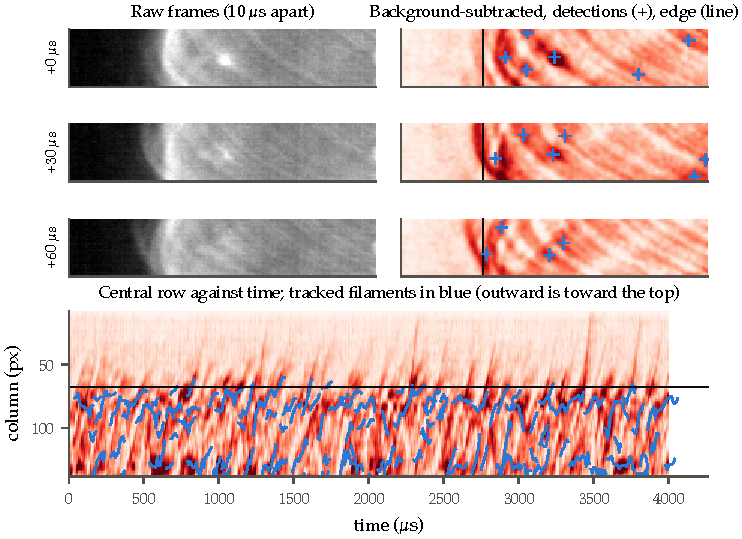
\includegraphics[width=\linewidth]{figs/fig_overview.pdf}
\caption{Pipeline stages on discharge 15235 (M6, 7~$\mu$s exposure), with three raw frames 30~$\mu$s apart and the corresponding background-subtracted frames with detections (crosses) and the edge column (line) in the top row, and the central row of the background-subtracted strip against time with tracked filaments overlaid in the bottom row, where filaments appear as inclined streaks that move toward the SOL (upward in this view).}
\label{fig:overview}
\end{figure}

\subsection{Strip geometry and the plasma edge}
A recording is an array of $n$ frames of $48 \times 256$ pixels with 10-bit depth, whose columns run across the plasma edge so that the SOL occupies one end of the strip and the core the other, with the end depending on how the camera was mounted in that campaign. The row-averaged brightness profile $p(t, x)$ is smoothed over 200 frames (2~ms) in time and $\sigma = 2$ columns in space, and the darker outer quarter of the columns is taken as the SOL side, which fixes a sign $s = \pm 1$ such that outward motion is $s\,\mathrm{d}x/\mathrm{d}t$. The edge column $x_{\rm half}(t)$ is the first column, scanning from the SOL side, at which $p$ exceeds the midpoint between the dark level, defined as the mean of the ten outermost SOL-side columns, and the interior level, defined as the median over the columns 40--75\% of the way across the strip from the SOL side, with linear sub-pixel interpolation. The limb peak $x_{\rm peak}(t)$ is the maximum of $p$ within 40 columns inboard of $x_{\rm half}$, refined by parabolic interpolation, and detections are referenced to $x_{\rm half}$ during processing and shifted to $x_{\rm peak}$ at aggregation, because the peak is the feature that the calibration in Section~\ref{sec:calibration} ties to the equilibrium.

\subsection{Background subtraction and detection}
Because filaments are transient, a per-pixel running minimum over 21 frames ($\pm 10$ frames, $\pm 100~\mu$s) estimates the quiescent background \citep{kirk2016filaments}, and the fluctuation image is the frame minus this background, passed through a $3 \times 3$ median filter and a Gaussian with $\sigma = 1$ pixel. The noise level $\sigma_n$ is $1.4826$ times the median absolute deviation of all fluctuation pixels in a block of 3{,}000 frames, pixels above $3\sigma_n$ are labelled into 8-connected components, and components smaller than 12 pixels are dropped. Each remaining component yields its intensity-weighted centroid $(x_c, y_c)$, its peak fluctuation, its orientation and major and minor axis lengths from its second central moments, and its radial width, which is measured on a chord as the number of columns at or above half the maximum of the fluctuation averaged over the five rows centred on $y_c$. The width is measured on a chord because filaments appear as inclined streaks and the column extent of a whole component grows with the tilt, and the signed SOL distance of a detection is $s\,(x_c - x_{\rm half})$.

\subsection{Tracking}
Detections in consecutive frames are linked by the Hungarian method \citep{kuhn1955hungarian}, with the Euclidean distance between centroids as the cost and a gate of 12 pixels per frame, which corresponds to about 4.5~cm or 4.5~km/s at the calibrated scale. Unmatched detections start new tracks, a track ends at the first frame without a match, and tracks with fewer than five detections (50~$\mu$s) are discarded. The radial velocity of a track in pixels per frame is the least-squares slope of $s\,x_c$ against frame index, with a standard error from the residuals, while its width is the median chord FWHM over the track and its SOL distance the median signed distance. Recordings are processed in blocks of 3{,}000 frames with a 60-frame overlap, and tracks that start in the overlap are dropped from the earlier block and recovered in the later one.

\subsection{Optical flow as an independent velocity}
As a check on the tracking, the velocity at each detection is also estimated by Lucas--Kanade optical flow \citep{lucas1981iterative}, in which Sobel spatial gradients and the frame difference in a $7 \times 7$ window around the centroid give a $2 \times 2$ least-squares system for the displacement between frames $f$ and $f + 1$, solved when its condition number is below $10^4$. The flow velocity of a track is the mean of the horizontal component over its detections with the sign $s$ applied, and because this estimate uses no assignment step and responds to the whole brightness profile around the centroid, agreement between the two estimates is evidence that neither is an artefact of its method.

\subsection{ELM detection}
Edge-localized modes (ELMs) eject large filaments that would dominate a velocity distribution, so they are detected from the midplane $D_\alpha$ monitor, sampled at 50--250~kHz depending on the campaign, as spikes where the residual after a 5~ms running median exceeds six times its robust standard deviation, with the time of each spike taken as the centre of mass of its samples. In some campaigns the monitor is coarsely digitized, with only tens of distinct values, which makes the robust standard deviation vanish, so the threshold is floored at six digitizer steps and at half the inter-ELM level. Because the $D_\alpha$ channel is absent or saturated in some discharges, the same detector is also applied to the frame-mean camera brightness, and a track that begins within 1~ms of a spike of either kind is flagged, while discharges with more than five $D_\alpha$ spikes inside the camera window are labelled ELMy. Flagged tracks are excluded from all statistics, and the parameter dependences in Section~\ref{sec:analysis} use the non-ELMy discharges only.

\subsection{Pixel scale from the equilibrium}
\label{sec:calibration}
The archive gives no spatial calibration for the strip recordings, and the scale is therefore recovered from the data. Because the limb peak sits where the line of sight is tangent to the flux surfaces at the LCFS, its sensor column should move with the outboard LCFS radius $R_{\rm LCFS}$ from EFIT, and the slope of column on radius is the inverse pixel scale. Within a single discharge $R_{\rm LCFS}$ moves by only a few centimetres during the flat top, the EFIT reconstruction is least reliable during ramp-up and termination, and the brightness profile changes shape as the density rises, so a within-shot regression is unstable (Appendix~\ref{app:calibration}). Between discharges, by contrast, the plasma position varies by 10--20~cm while the camera and its optics stay fixed through a campaign, which gives a much longer lever arm.

For each discharge, $R_{\rm LCFS}$ is taken at every EFIT time inside the flat top as the largest major radius of the EFIT boundary contour within 5~cm of the magnetic-axis height, $x_{\rm peak}$ is taken from the profile smoothed over 2~ms, and EFIT samples whose $R_{\rm LCFS}$ differs by more than 8~cm from the flat-top median are dropped as unconverged. Each discharge then contributes one point, its median $x_{\rm peak}$, converted to sensor coordinates by adding the region-of-interest offset recorded in the camera metadata, against its median $R_{\rm LCFS}$. A camera configuration is defined as the combination of campaign, view string in the camera metadata, and region-of-interest offset, because a change in any of these can mean a change of lens, pointing, or sensor region. A configuration with at least 8 discharges and at least 3~cm of spread in $R_{\rm LCFS}$ receives its own Theil--Sen slope \citep{sen1968estimates}, which is kept if its sign agrees with $s$, the Spearman correlation satisfies $|\rho| \ge 0.5$, and the bootstrap interval excludes zero. Every other configuration uses the pooled slope of its campaign, fitted on all configurations of the campaign after the mean $R_{\rm LCFS}$ and mean column of each configuration are subtracted to remove the per-configuration intercepts, and in all cases the 95\% intervals come from 2{,}000 bootstrap resamples of discharges within configurations \citep{efron1993bootstrap} and the scale is the inverse of the slope magnitude.

\subsection{Physical units and track selection}
The radial velocity of a track is $v_r = s\,\dot x_c \times f_{\rm frame} \times \ell$, where $\ell$ is the pixel scale, and its radial width is $\delta_r = \mathrm{FWHM} \times \ell$, while the SOL distance is measured from $x_{\rm peak}$ using the per-shot median offset $x_{\rm peak} - x_{\rm half}$. A track enters the statistics if its median position lies between 10 pixels inboard and 40 pixels outboard of the limb peak (3--5~cm inboard to 11--21~cm outboard, depending on the scale of the configuration), its velocity standard error is below 0.5 pixels per frame, its width is finite, it begins inside the plasma flat top, and it is free of an ELM flag. A discharge enters the shot-level statistics if it has at least 50 such tracks with $v_r > 0$, which keeps the per-discharge medians stable.

\subsection{Statistics}
All central values are medians with 95\% bootstrap intervals from 2{,}000 resamples, and slopes are Theil--Sen estimates in $\log_{10}$--$\log_{10}$ coordinates with the 95\% interval of the estimator, reported together with Spearman's $\rho$. The velocity--size slope is computed per discharge and also pooled, and for the pooled fit the $v_r$ and $\delta_r$ of each track are divided by the medians of its discharge so that differences between discharges in the pixel scale or the plasma conditions do not create a spurious correlation. The correction for exposure blur replaces $\delta_r$ by $\delta_{\rm corr} = (\delta_r^2 - (v_r t_{\rm exp})^2)^{1/2}$, which treats the smear as a Gaussian of width $v_r t_{\rm exp}$ added in quadrature, before the slope is refitted. Parameter dependences are Theil--Sen slopes of the per-discharge median $v_r$ and $\delta_r$ on plasma current, Greenwald fraction, and injected beam power, with the beam power offset by 0.05~MW so that Ohmic discharges enter the log fit.

The two-region normalization requires $T_e$ and $n_e$ at the LCFS, $B$, $q_{95}$, and $R$, and the temperature comes from the Thomson scattering profile, from the edge system where it exists and the core system otherwise, interpolated at $R_{\rm LCFS}$ and taken as the median over the flat top, with $T_e = \teDefault$~eV assumed and marked as such when no profile reaches the LCFS. The separatrix density $n_{e,\rm sep}$ is taken as half the line-averaged density, $B$ as the vacuum toroidal field at the magnetic axis scaled by $R_{\rm axis}/R_{\rm LCFS}$, and the connection length as $L_\parallel = \pi q_{95} R_{\rm axis}$, while the filament radius in the model is half the measured FWHM, $a = \delta_r/2$, and $\nu_{ei}$ follows the NRL formulary \citep{nrl2019formulary} with deuterium ions.

\section{Results}
\label{sec:results}


\subsection{Pixel scale}
Of the \nConfigs{} camera configurations listed in Table~\ref{tab:configs} in the appendix, \nConfigsOwn{} have enough discharges and enough spread in $R_{\rm LCFS}$ for their own fit and cover \nShotsOwnScale{} of the \nShotsProcessed{} processed discharges, while the rest use the pooled slope of their campaign (Figure~\ref{fig:calibration}). The limb-peak column falls linearly with $R_{\rm LCFS}$ in every fitted configuration, with Spearman correlations between \scaleOwnRhoWeak{} and \scaleOwnRhoStrong{}, the sign of every slope agrees with the SOL direction found from the images, and the fitted scales span \scaleOwnMin{}--\scaleOwnMax{}~mm per pixel. The tightest fit is the M6 configuration ``\scaleCfgCampSixView'' (\scaleCfgCampSixN{} discharges, $\rho = \scaleCfgCampSixRho$), at \scaleCfgCampSix{}~mm per pixel (\scaleCfgCampSixLo--\scaleCfgCampSixHi), and the M9 configuration gives \scaleCfgCampNine{}~mm per pixel (\scaleCfgCampNineLo--\scaleCfgCampNineHi). For the same camera, port, and campaign, \citet{farley2019identification} quote a resolution of 5~mm at the tangency plane for wide-angle images reduced to $256 \times 160$ pixels from the $640 \times 448$ mode of the camera, which is about 2~mm per native pixel, so the M9 value is of that order, although 2~mm lies below its interval and the archive does not record whether the lens was the same.

Two features of the calibration limit what the physical units can support, the first being that the intervals are 10--30\% wide and cannot capture a bias common to a whole configuration, such as a drift of the emission peak relative to the LCFS with density. The second is that the filaments look alike in pixel units in every configuration, since across the \nCfgPx{} fitted configurations with at least ten discharges the median track velocity is \vxPxCfgMin{}--\vxPxCfgMax{} pixels per frame and the median width is \fwhmPxCfgMin{}--\fwhmPxCfgMax{} pixels, while the fitted scales differ by a factor of \scaleOwnRatio. The differences between campaigns in Table~\ref{tab:campaigns} therefore reflect differences between their calibrations and are left uninterpreted. Because a scale error multiplies $v_r$ and $\delta_r$ of a configuration by the same factor, it cancels in the velocity--size slopes of Section~\ref{sec:analysis}, which are fitted after each discharge is normalized by its own medians, and it moves a discharge along a diagonal in the regime diagram without changing the conclusions drawn there.

\begin{figure}[t]
\centering
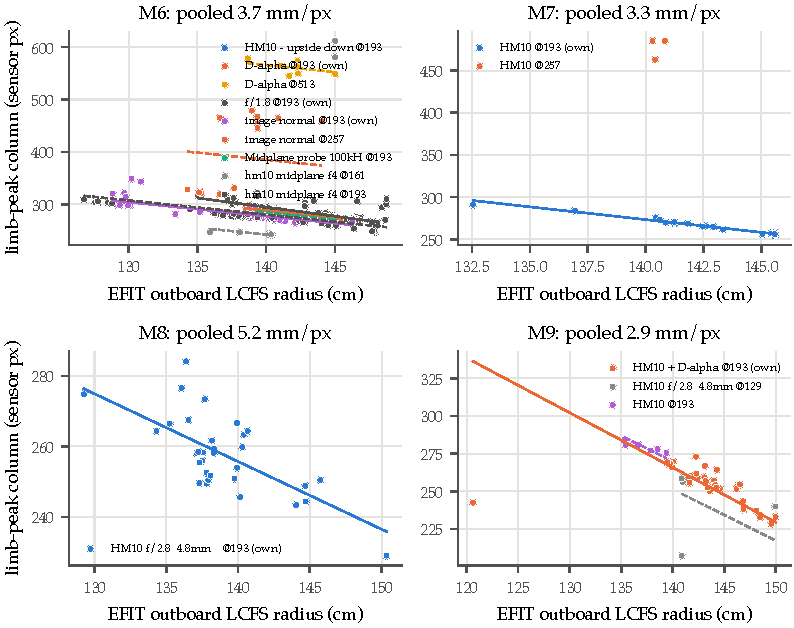
\includegraphics[width=\linewidth]{figs/fig_calibration.pdf}
\caption{Between-shot pixel-scale calibration, in which each point is one discharge, placed at its median limb-peak column in sensor coordinates over the flat top against its median EFIT outboard LCFS radius. Colours mark camera configurations (view string and region-of-interest offset), solid lines show the Theil--Sen fit of each configuration, dashed lines show the pooled campaign slope with the intercept of the configuration, and the scale is the inverse of the slope.}
\label{fig:calibration}
\end{figure}

\subsection{Velocity and width distributions}
The statistics include the \nShotsStats{} discharges with at least 50 selected tracks, \nTracksSel{} tracks in total, and Figure~\ref{fig:distributions} shows the pooled distributions, with a median radial velocity over discharges of \vMedAll{}~m/s (95\% interval \vMedAllLo--\vMedAllHi) and a median radial width of \dMedAll{}~cm (\dMedAllLo--\dMedAllHi). The velocity distribution is skewed with a tail to 2--3~km/s, and the width distribution peaks at 2--3~cm with a tail to 10~cm. Among all near-edge tracks that pass the quality cuts, \outwardMed\% move outward, and the inward-moving remainder is concentrated inboard of the limb peak, where the field-aligned streaks sweep across the strip as they rotate with the plasma, so only outward-moving tracks enter the velocity--size analysis.

\begin{figure}[t]
\centering
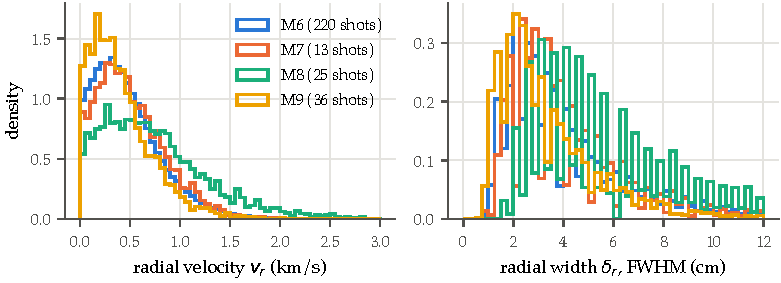
\includegraphics[width=\linewidth]{figs/fig_distributions.pdf}
\caption{Distributions of radial velocity (left) and radial FWHM (right) of the selected tracks in each campaign, pooled over the discharges in the statistics.}
\label{fig:distributions}
\end{figure}

\subsection{Independent velocity estimates}
Two estimates that do not use the tracking confirm the velocity scale, the first being the cross-correlation lag between the row-averaged fluctuation profiles of consecutive frames inside the near-edge window, which involves no detection step and gives a per-discharge median velocity of \xcorrVMed{}~m/s over the \nXcorr{} discharges in which more than half the frame pairs have a usable correlation peak. Its ratio to the tracking median is \xcorrRatioMed{} (\xcorrRatioLo--\xcorrRatioHi), and the two correlate across discharges with Spearman $\rho = \xcorrShotRho$, while a ratio below one is expected because the lag method weights every bright structure in the window, including the slow inboard part of the streaks and the stationary limb. The second, Lucas--Kanade flow at the detections, correlates with the track velocities within discharges, with a median per-discharge correlation of \lkAgreeMed{} and $\rho = \lkShotRho$ between discharge medians, but is smaller by a factor of \lkRatioMed. Because the streaks are elongated and inclined, the brightness-constancy constraint fixes only the component of motion normal to the streak, and displacements exceed one pixel per frame, both of which bias the flow magnitude down, so the flow serves only as a check on sign and ordering.

\section{Analysis}
\label{sec:analysis}

\subsection{Velocity against size}
Figure~\ref{fig:vd} shows the velocity--size relation after each discharge is normalized by its own medians. The per-discharge Theil--Sen slope of $\log v_r$ on $\log \delta_r$ has a median of \vdSlopeMed{} (\vdSlopeMedLo--\vdSlopeMedHi) and is positive in \vdSlopePosShare\% of discharges; the pooled slope is \vdSlopePooled{} (\vdSlopePooledLo--\vdSlopePooledHi) with Spearman $\rho = \vdRhoPooled$. The relation is far from both limiting scalings: the sheath-connected $\delta^{-2}$ is excluded, and the inertial $\delta^{1/2}$ lies well above the interval.

\begin{figure}[t]
\centering
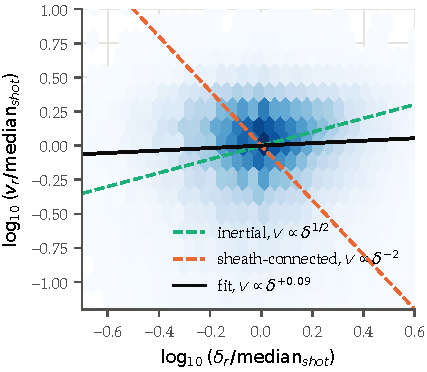
\includegraphics[width=0.55\linewidth]{figs/fig_vd.pdf}
\caption{Radial velocity against radial width, each normalized by the median of its discharge, for all selected tracks (hexagonal bin density). The solid line is the pooled Theil--Sen fit; dashed lines are the sheath-connected and inertial scalings through the medians.}
\label{fig:vd}
\end{figure}

\subsection{Exposure blur}
A filament that moves during the exposure is smeared along its direction of motion, and faster filaments are smeared more, which produces a positive velocity--width correlation with no physical content. The median smear $v_r t_{\rm exp}$ is \blurMedCm{}~cm, about a tenth of the median width, so the effect is small but not negligible. Two tests bound it. First, the slope depends on exposure in the expected direction within M6, where the two common settings share the optics: the per-discharge slope has a median of \vdSlopeExpSeven{} (\vdSlopeExpSevenLo--\vdSlopeExpSevenHi) at 7~$\mu$s ($n = \nExpSeven$) and \vdSlopeExpTen{} (\vdSlopeExpTenLo--\vdSlopeExpTenHi) at 10~$\mu$s ($n = \nExpTen$), while the median width is the same, \dMedExpSeven{} against \dMedExpTen{}~cm, because the extra smear of 3~$\mu$s at 400~m/s is 0.1~cm. The 4~$\mu$s discharges belong to M7 and M8 and are not comparable in width, but their slope, \vdSlopeExpFour{} (\vdSlopeExpFourLo--\vdSlopeExpFourHi), is also low.
Second, correcting each width for its own smear in quadrature lowers the pooled slope to \vdSlopePooledBlur{} (\vdSlopePooledBlurLo--\vdSlopePooledBlurHi). We take this corrected value as the measurement: the radial velocity is nearly independent of width over the measured range, with at most a weak positive dependence.

\begin{figure}[t]
\centering
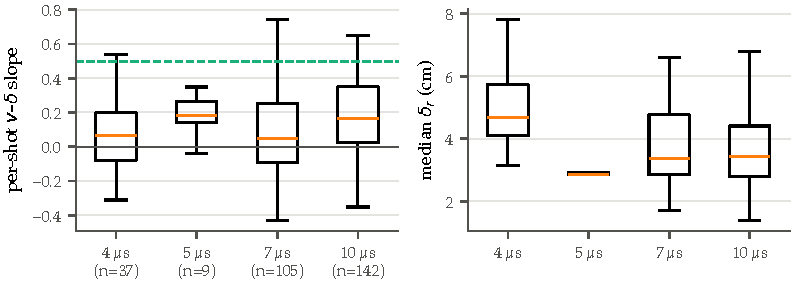
\includegraphics[width=\linewidth]{figs/fig_exposure.pdf}
\caption{Effect of exposure time. Left: per-discharge velocity--width slopes by exposure setting; the dashed line is the inertial scaling. Right: per-discharge median width by exposure.}
\label{fig:exposure}
\end{figure}

\subsection{Two-region normalization}
With the inputs of Section~\ref{sec:method}, the median reference scales are $a^* = \aStarMed$~cm, $v^* = \vStarMed$~m/s, and $\Lambda = \LambdaMed$, so the discharges sit in the low-collisionality half of the regime diagram. Figure~\ref{fig:regimes} places each discharge at its median $\hat a = (\delta_r/2)/a^*$ and $\hat v = v_r/v^*$. The filaments span $\hat a = \aHatMin$--$\aHatMax$ (median \aHatMed), which straddles the velocity maximum of the model; over the central half of this range the model's $\hat v(\hat a)$ stays within a factor of two of its peak. A sample that straddles the peak is expected to show a weak net dependence of velocity on size, and this is what we measure. The normalized velocity, however, is $\hat v \approx \vHatMed$: the measured filaments move at a few percent of the model's velocity scale. Part of this gap is the input assumptions, since $v^* \propto T_e^{7/10}$ and $T_e$ at the LCFS is assumed for \nTeAssumed{} of the \nShotsStats{} discharges, and part is the model itself, which gives the velocity of an isolated, fully formed filament with an order-unity prefactor that simulations in realistic geometry find to be below one \citep{walkden2015characterization, paruta2018blob}. The measurement is also made within 15~cm of the limb, where filaments are still forming and accelerating. The ratio is nonetheless larger than the prefactor uncertainty alone explains, and we regard the amplitude, not the size dependence, as the point of tension with the model.

\begin{figure}[t]
\centering
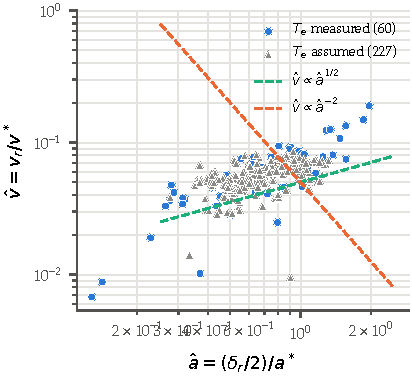
\includegraphics[width=0.55\linewidth]{figs/fig_regimes.pdf}
\caption{Per-discharge median velocity and size in two-region units. Dashed lines are the inertial ($\hat v = \hat a^{1/2}$) and sheath-connected ($\hat v = \hat a^{-2}$) branches. Circles use a measured $T_e$ at the LCFS; triangles assume $T_e = \teDefault$~eV.}
\label{fig:regimes}
\end{figure}

\subsection{Dependence on plasma parameters}
Figure~\ref{fig:params} shows the per-discharge medians against plasma current and Greenwald fraction for the \nShotsL{} non-ELMy discharges, which span $I_p = \ipMin$--\ipMax{}~kA and $f_{\rm GW} = \fgwMin$--\fgwMax. No dependence is resolved. The log--log slope of the median velocity on plasma current is \slVIp{} (\slVIpLo--\slVIpHi) and on Greenwald fraction \slVFgw{} (\slVFgwLo--\slVFgwHi); for the width the slopes are \slDIp{} (\slDIpLo--\slDIpHi) and \slDFgw{} (\slDFgwLo--\slDFgwHi). Beam power has no effect on the velocity (\slVNbi, \slVNbiLo--\slVNbiHi) and a small positive one on the width (\slDNbi, \slDNbiLo--\slDNbiHi). Because these fits pool configurations with different calibrations, we repeat them inside the best-calibrated configuration alone (``\bestCfgView'', \nShotsBestCfgL{} non-ELMy discharges at one scale, $I_p = \ipBestMin$--\ipBestMax{}~kA): the velocity slopes are \slBVIp{} (\slBVIpLo--\slBVIpHi) on current and \slBVFgw{} (\slBVFgwLo--\slBVFgwHi) on Greenwald fraction, consistent with the pooled result.
\citet{kirk2016filaments} found in a dedicated current scan at fixed density and power that the radial velocity falls with current. Our sample is not a controlled scan: current, density, heating, and campaign vary together, and most discharges sit near 700~kA, so a weak dependence is within the reach of confounding. We report the slopes as they are and do not claim a contradiction.

\begin{figure}[t]
\centering
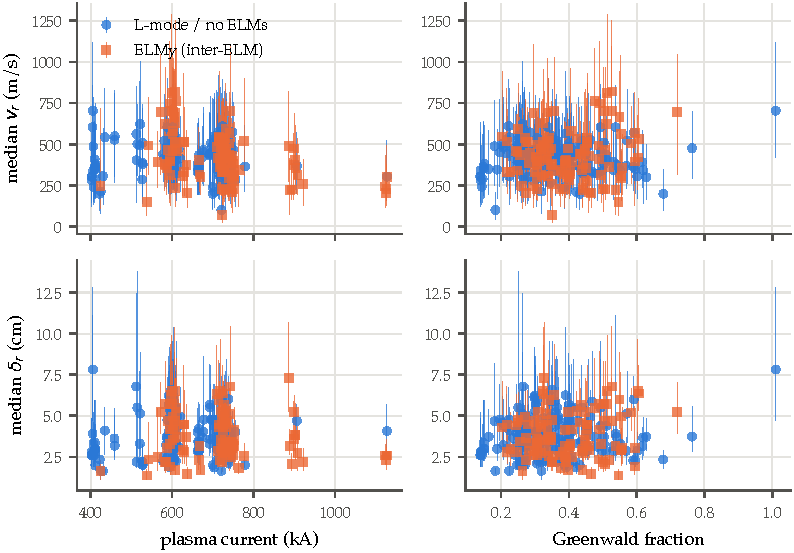
\includegraphics[width=\linewidth]{figs/fig_params.pdf}
\caption{Per-discharge median radial velocity (top) and width (bottom) against plasma current (left) and Greenwald fraction (right). Bars are interquartile ranges over tracks. Circles are discharges without ELMs in the camera window; squares are ELMy discharges, measured between ELMs.}
\label{fig:params}
\end{figure}

\section{Related Work}
\label{sec:related}

\paragraph{Filament imaging on MAST.}
\citet{dudson2008experiments} used the midplane fast camera with automated analysis of L-mode images and BOUT simulations. They found that the toroidal mode number of the edge turbulence rises with density and falls with $q_{95}$, that filament width has the opposite dependence, and that simulated filaments are born within about 2~cm of the edge in a self-generated $E \times B$ shear layer. \citet{benayed2009interelm} combined camera images with a reciprocating Langmuir probe during inter-ELM periods and showed that filaments rotate near the LCFS and move outward, with more and faster filaments at higher density; they used the radial velocities to test the sheath-connected and inertial scalings. \citet{kirk2016filaments} scanned the plasma current at fixed density and heating power in L-mode and found that the radial velocity, and to a lesser extent the radial size, decrease as the current rises, and that this dependence is consistent with the measured divertor profiles. \citet{farley2019identification} introduced a tomographic inversion of wide-angle images onto a basis of equilibrium field lines, which turns filament identification into a problem in field-aligned coordinates. All of these studies relied on a camera geometry model built with Calcam \citep{silburn2018calcam} for the view in use. The present work differs in three ways: it uses the 48-row strip mode at 100~kHz rather than wide-angle frames, it recovers the pixel scale from the equilibrium instead of a geometry model, and it processes hundreds of discharges across four campaigns rather than a scan of a few.

\paragraph{Blob theory and simulation.}
The sheath-connected scaling is due to \citet{krasheninnikov2001scrape} and the inertial scaling to \citet{garcia2006fluctuations}. \citet{myra2006collisionality} introduced the two-region model that we use for normalization; \citet{dippolito2011convective} review the model and its comparisons with experiment. \citet{theiler2009blob} measured the velocity--size relation on TORPEX and recovered the predicted regime transitions. Three-dimensional simulations of isolated filaments \citep{easy2014three, walkden2015characterization, paruta2018blob} find that the scalings hold in form but that realistic geometry and parallel dynamics change the prefactors. \citet{zweben2007edge} review edge turbulence imaging across devices, including the relation between light emission and density fluctuations that imaging measurements rely on.

\paragraph{Methods.}
The detection and tracking steps are standard: connected-component labelling after robust thresholding, frame-to-frame assignment by the Hungarian method \citep{kuhn1955hungarian}, and Lucas--Kanade optical flow \citep{lucas1981iterative}. Slopes use the Theil--Sen estimator \citep{sen1968estimates} and confidence intervals use the bootstrap \citep{efron1993bootstrap}. The data come from the FAIR-MAST archive \citep{jackson2024fairmast}.

\section{Limitations}
\label{sec:discussion}

\paragraph{Calibration.}
The pixel scale rests on the assumption that the limb peak tracks the EFIT outboard LCFS radius with a fixed offset within a camera configuration. The offset can drift with the emission profile, which depends on density and neutral pressure, and EFIT's boundary carries its own uncertainty of order a centimetre. The bootstrap intervals in Table~\ref{tab:configs} include the scatter these effects produce but not a common bias. The near-uniformity of the filaments in pixel units across configurations whose fitted scales differ by almost a factor of two (Section~\ref{sec:results}) is either a coincidence or a sign that part of the spread in the fitted scales is not optical; we cannot decide this from the archive, and we have therefore drawn no conclusion that depends on comparing physical units between configurations. Every velocity and width in the paper should be read with a systematic uncertainty of 10--30\% in its configuration's scale, and a comparison between configurations with up to a factor of two. A per-shot Calcam model would remove this uncertainty and is the natural next step if the calibration images can be released. Appendix~\ref{app:calibration} shows why the within-shot regression is not a substitute.

\paragraph{Geometry.}
The strip gives a single row band through the edge. The column axis is close to radial only at the tangency plane, and the width we measure is the chord length of an inclined streak, which overestimates the width perpendicular to the filament by $1/\cos\theta$ with $\theta$ the streak angle to the column axis. We do not correct for this, because the angle is poorly determined in a 48-row strip; the effect inflates $\delta_r$ by a factor that is roughly constant within a campaign and therefore shifts $\hat a$ but not the velocity--size slope. Emission is line-integrated along the view, so a bright structure behind the tangency plane projects to a smaller apparent radius; this blurs the SOL distance but not the velocity, which is a time derivative.

\paragraph{What the camera sees.}
$D_\alpha$ emission depends on neutral density as well as plasma density, and the neutral density falls steeply inside the LCFS. Filaments are therefore visible mainly in the SOL, and a filament's brightness changes as it moves. Tracking by centroid is robust to a slowly changing amplitude; optical flow is not, which is one reason the flow velocities are low.

\paragraph{Selection.}
We measure between 10 pixels inboard and 40 pixels outboard of the limb, that is from 3--5~cm inboard to 11--21~cm outboard depending on the configuration, a region that includes filaments at birth. Velocities in the far SOL may differ. The 50-track threshold per discharge and the exclusion of ELM-adjacent tracks remove some discharges and some of the largest events; the headline numbers describe inter-ELM and L-mode filaments near the edge.

\paragraph{Model inputs.}
$T_e$ at the LCFS is assumed for most discharges, and $n_{e,\rm sep}$ is taken as half the line average. Both enter $a^*$, $v^*$, and $\Lambda$ as power laws with exponents below one, so a factor of two in either moves a discharge by less than a factor of two in the regime diagram. The conclusion that the sample straddles $\hat a = 1$ is robust to this; the value of $\hat v$ is not better than a factor of two.

\section{Conclusion}
\label{sec:conclusion}
Public archives make it possible to measure filament statistics on hundreds of discharges with a pipeline that no one tunes by hand. On MAST, the 100~kHz strip recordings give radial velocities and widths for \nTracksSel{} filaments in \nShotsStats{} discharges, with a pixel scale recovered from the equilibrium for each camera configuration to 10--30\%. The radial velocity has a median of \vMedAll{}~m/s and does not depend on filament width to within a log--log slope of about 0.1 once exposure blur is removed. In two-region units the filaments sit around the predicted velocity maximum, which explains the flat dependence, but they move at a few percent of the model's velocity scale. The amplitude discrepancy, the campaign-level calibration, and the radial-only geometry are the three places where a dedicated experiment or a released geometry model would improve on what the archive alone can give.


\section*{Acknowledgements}
I thank the professors who teach computer vision at Stanford, notably Juan Carlos Niebles, Adrien Gaidon, and Silvio Savarese; their courses led me to the ideas behind this work.

\bibliography{refs}
\bibliographystyle{colm2026_conference}

\clearpage
\appendix
\section{Camera configurations}
\label{app:views}
Table~\ref{tab:configs} lists the camera configurations in the processed set: the view string from the camera metadata, the sensor column offset of the region of interest, the number of discharges, the spread of $R_{\rm LCFS}$ across the discharges, the Spearman correlation between limb-peak column and $R_{\rm LCFS}$, the configuration's own scale where it could be fitted, and whether the configuration uses its own scale or the pooled campaign scale (Section~\ref{sec:calibration}).

\begin{table}[h]
\centering
\scriptsize
\setlength{\tabcolsep}{4pt}\begin{tabular}{llrrrlll}
\toprule
Camp. & View string & ROI left & Shots & $\Delta R_{\rm LCFS}$ (cm) & $\rho$ & Scale (mm/px) & Used \\
\midrule
M6 & HM10, normal, f/1.8 & 193 & 70 & 13 & -0.94 & 2.9 (2.7--3.0) & own \\
M6 & HM10, normal & 193 & 61 & 17 & -0.89 & 3.7 (3.1--4.1) & own \\
M6 & hm10 midplane f4 & 193 & 59 & 22 & -0.47 & 3.9 (3.6--5.1) & pooled \\
M6 & HM10, normal, D$\alpha$ 10 nm & 193 & 30 & 7 & -0.88 & 3.5 (3.2--3.9) & own \\
M6 & HM10, normal & 257 & 14 & 10 & +0.34 & 0.9 (0.4--1.9) & pooled \\
M6 & HM10, normal, D$\alpha$ 10 nm & 513 & 7 & 6 & -- & -- & pooled \\
M6 & hm10 midplane f4 & 161 & 6 & 4 & -- & -- & pooled \\
M6 & HM10 - upside down & 193 & 3 & 1 & -- & -- & pooled \\
M6 & probe 100kHz & 193 & 3 & 6 & -- & -- & pooled \\
M6 & HM10, normal, D$\alpha$ 10 nm & 545 & 2 & 0 & -- & -- & pooled \\
M6 & HM10, normal, D$\alpha$ 10 nm & 225 & 1 & 0 & -- & -- & pooled \\
M6 & HM10, normal & 225 & 1 & 0 & -- & -- & pooled \\
M6 & probe view & 193 & 1 & 0 & -- & -- & pooled \\
M7 & HM10 & 193 & 22 & 13 & -0.88 & 3.3 (3.0--3.8) & own \\
M7 & HM10 & 257 & 3 & 1 & -- & -- & pooled \\
M8 & HM10 f/2.8 4.8mm nd 0.9 & 193 & 32 & 21 & -0.58 & 5.2 (3.6--11.5) & own \\
M9 & HM10 + D$\alpha$ filter & 193 & 38 & 29 & -0.82 & 2.7 (2.5--3.4) & own \\
M9 & HM10 & 193 & 6 & 4 & -- & -- & pooled \\
M9 & HM10 f/2.8 4.8mm & 129 & 4 & 9 & -- & -- & pooled \\
M9 & HM10 + D$\alpha$ filter & 129 & 1 & 0 & -- & -- & pooled \\
M9 & HM10 + D$\alpha$ filter & 513 & 1 & 0 & -- & -- & pooled \\
M9 & HM10 + D$\alpha$ filter & 577 & 1 & 0 & -- & -- & pooled \\
M9 & HM10 & 129 & 1 & 0 & -- & -- & pooled \\
\bottomrule
\end{tabular}

\caption{Camera configurations and their calibration. A configuration uses its own scale when it has at least 8 discharges, at least 3~cm of spread in $R_{\rm LCFS}$, a correlation of the right sign with $|\rho| \ge 0.5$, and a bootstrap interval that excludes zero.}
\label{tab:configs}
\end{table}

\section{Within-shot calibration}
\label{app:calibration}
A within-shot regression of the limb-peak column on $R_{\rm LCFS}$ uses the few centimetres of plasma movement during a flat top. For the \nWithinShot{} discharges in which the LCFS moves by at least 2~cm, the implied scale has a median of \withinScaleMed{}~mm per pixel with an interquartile range of \withinScaleQLo--\withinScaleQHi{} and extremes below 1 and above $10^{\withinScaleMaxLog}$. The spread comes from three effects: the EFIT boundary is least reliable at the start and end of the flat top, where most of the movement occurs; the brightness profile changes shape as the density rises, which moves the peak at fixed $R_{\rm LCFS}$; and the lever arm is short, so a 1~cm error in $R_{\rm LCFS}$ changes the slope by tens of percent. The between-shot regression of Section~\ref{sec:calibration} replaces a few centimetres of movement in one discharge with 10--20~cm of position variation across a campaign and is correspondingly more stable.

\section{ELM detection}
\label{app:elm}
Figure~\ref{fig:elm} shows the $D_\alpha$ trace and the camera frame-mean brightness for an ELMy discharge, with the detected spikes. The camera proxy finds the same events as the $D_\alpha$ monitor where both are available and serves as the only detector where the $D_\alpha$ channel is missing.

\begin{figure}[h]
\centering
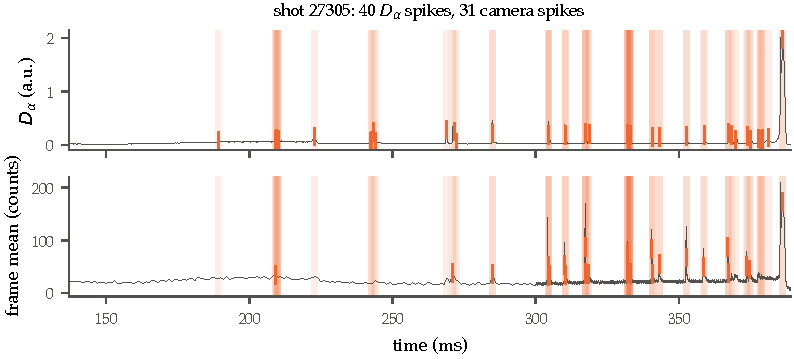
\includegraphics[width=\linewidth]{figs/fig_elm.pdf}
\caption{ELM detection on an ELMy discharge. Top: midplane $D_\alpha$ with detected spikes marked. Bottom: camera frame-mean brightness with its own spike detection. The shaded bands are the $\pm 1$~ms exclusion windows.}
\label{fig:elm}
\end{figure}


\end{document}
